\begin{figure}[ht] 
 	\centering 
 	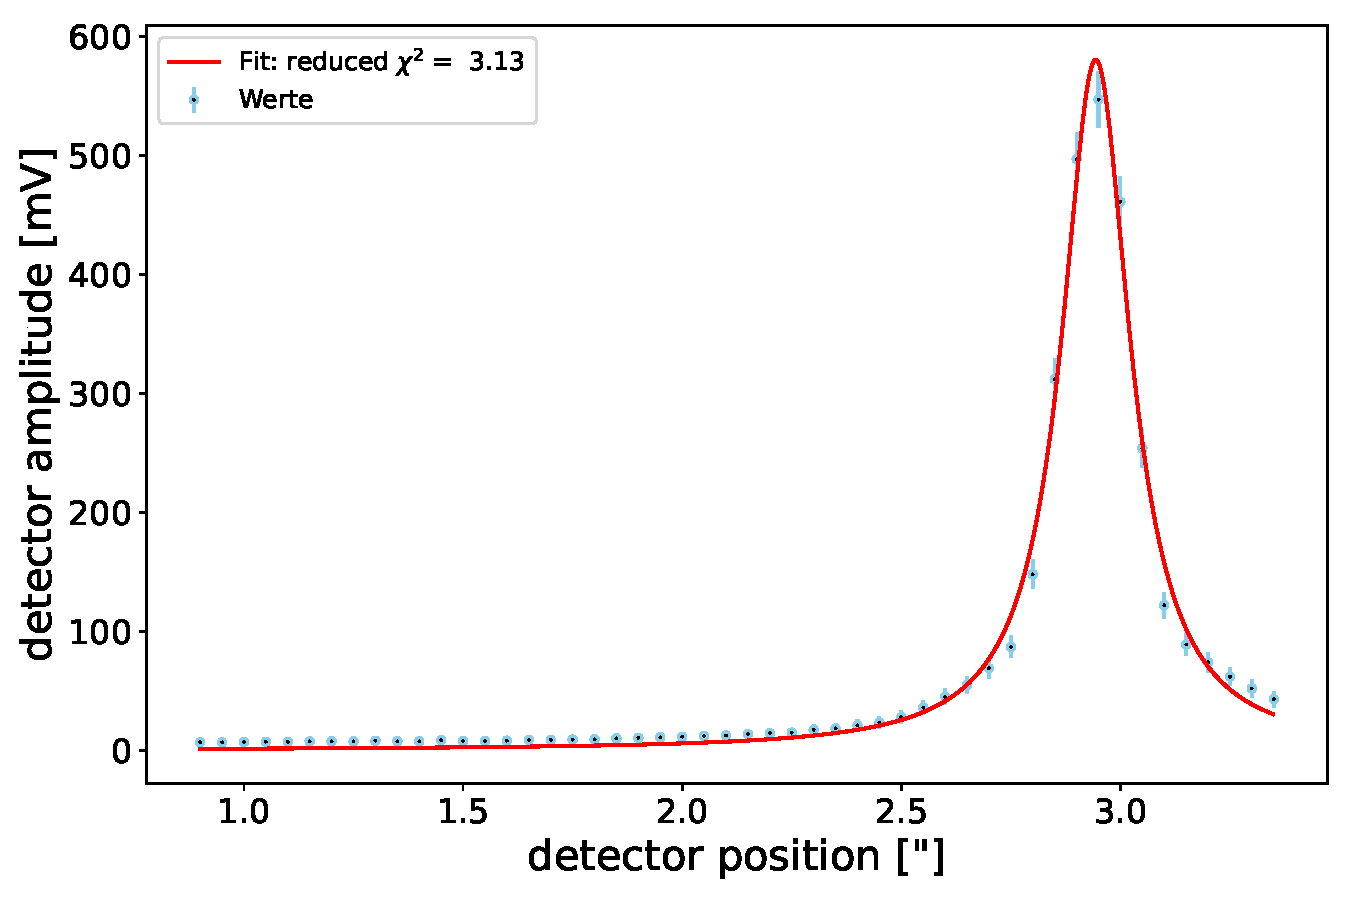
\includegraphics[width= 0.65 \textwidth]{Fits/Amps_B0A_Fit.pdf} 
	\caption{Amps_B0A, Fit} 
 	\label{fig:Amps_B0A, Fit} 
\end{figure}
 \\ 
\begin{table}[ht] 
\centering 
\caption{Amps_B0A, Fit Parameter Tabelle} 
\label{tab:my-table}
\begin{tabular}{|l|c|}
\hline
Parameter Name	&	Wert \\ \hline
amplitude	&	 173.781 \pm  5.538\\ \hline
center	&	 2.944 \pm  0.00402\\ \hline
sigma	&	 0.0954 \pm  0.0089\\ \hline
fraction	&	 0.998 \pm  0.0129\\ \hline
fwhm	&	 0.191 \pm  0.0178\\ \hline
height	&	 580.549 \pm  60.600\\ \hline
\end{tabular} 
\end{table}